\chapter*{Introducción}
\addcontentsline{toc}{chapter}{Introducción}

Al someter un liquido a vibraciones netamente verticales, se observa que en la superficie del liquido se presentan determinados patrones regulares definidos por un cierto rango de frecuencia y amplitudes de la frecuencia de excitación; a este fenómeno se le conoce como \textit{Inestabilidad de Faraday}. El estudio de este tipo de inestabilidad tiene una larga e interesante historia que involucra a dos de los científicos más destacados de la ciencia moderna. A mediados del año 1831, M. Faraday (1791-1867) realizó una serie de experimentos con fluidos sometidos a vibraciones verticales \cite{Faraday1831}. En su bitacora personal Faraday reportó que al hacer vibrar un fluido se presentan una serie de patrones cuadrados en su superficie ``Crispaciones casi siempre cuadrangulares, siempre cuando están bien formadas, pero modificadas por el borde del agua o el líquido, también por el centro de movimiento'' (Faraday, 1831) \cite{Martin1832}. En particular, Faraday señaló que la frecuencia de las ondas presentes en la superficie del liquido era la mitad de la frecuencia de excitación. Casi cuatro décadas después, L. Mathiessen cuestionó la respuesta subarmónica a las vibraciones puramente verticales \cite{Matthiessen1868}, argumentado la existencia de una sincronía entre el forzamiento y las ondas en la superficie del fluido. Esta controversia motivó a Lord Rayleigh (1842-1919) a hacer sus propios análisis, quien mediante un dispositivo bastante ingenioso pudo constatar la afirmación realizada por Faraday \cite{Rayleigh1883b}.\medskip

\begin{figure}
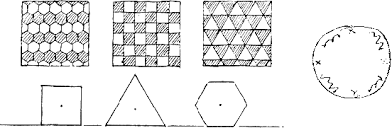
\includegraphics[scale=1]{figuras/faradaysketch.png}
\caption{Izquierda: Bocetos de patrones hexagonales, rectangulares y triangulares realizados por Faraday como posibles interpretaciones de la geometría de las crispaciones. Derecha: Diagrama de la vista superior realizada por Faraday de la distribución de crispaciones en un vaso de agua; ``x'' representa los lugares donde el de agua permanece inmóvil o las crispaciones son débiles, mientras que las líneas onduladas indican una superficie más agitada.\cite{Martin1832}} %sacado de Cavicchi
\end{figure}

En 1954, Benjamin y Ursell desarrollaron una teoría lineal sobre la naturaleza subarmónica de la inestabilidad, realizando la verificación teórica directamente de la hidrodinámica \cite{Benjamin1954}. Sin embargo, el análisis de Benjamin y Ursell se basa en una aproximación de flujo potencial, la cual está restringida únicamente a fluidos sin viscosidad. Si la inestabilidad es generada en un líquido viscoso, una parte de la energía mecánica es disipada debido a esta. Estos efectos generalmente se manejan agregando un amortiguamiento heurístico en la ecuación de Mathieu \cite{Landau1988}, que es proporcional a la viscosidad cinemática $\nu$. La inclusión de dicho término ha sido utilizado ampliamente en varios análisis lineales como los realizados por Müller \cite{Muller1993}; Kumar y Tuckerman \cite{Kumar1994}; Kumar \cite{Kumar1996} y Perlin y Schultz \cite{Perlin2000}. Sin embargo, esta aproximación ignora las capas límite viscosas a lo largo de las paredes del contenedor y debajo de la superficie, donde se produce una disipación adicional. \medskip

La descripción matemática completa del problema involucra las ecuaciones de Navier-Stokes en un dominio con una superficie libre, donde las amplitudes de los modos normales se desacoplan y cumplen en primera aproximación de la ecuación de Mathieu, la cual es una ecuación diferencial ordinaria de segundo orden no autónoma. En matemáticas, un sistema no autónomo es un sistema de ecuaciones diferenciales ordinarias que depende explícitamente de la variable independiente. En este caso, la falta de autonomía está dada por el forzamiento externo que influye en los parámetros del fluido cuando se inicia el comportamiento oscilante. Benjamin y Ursell pudieron utilizar las propiedades de estabilidad conocidas de la ecuación de Mathieu para confirmar el punto de vista de Faraday y Rayleigh. Al tipo de inestabilidad presente en la ecuación de Mathieu se le llama \textit{Inestabilidad paramétrica}, y es conocida por estar presente en diversos sistemas como osciladores electrónicos, ondas de Langmuir en plasma y hasta en el comportamiento estocástico de un conjunto de precios sectoriales internacionales. El experimento mas representativo de este fenómeno es el péndulo excitado paramétricamente. Si el pivote del péndulo oscila verticalmente, el péndulo comenzará a oscilar horizontalmente con la mitad de la frecuencia de excitación para algunas amplitudes y frecuencias. En este ejemplo, así como en el experimento de Faraday, la aceleración gravitacional efectiva es el parámetro externo impulsador. La ecuación de Mathieu lleva el nombre del matemático francés E. L. Mathieu (1825-1890), quien en su trabajo original de 1868 muestra como resolver la ecuación de onda bidimensional para el movimiento de una membrana elíptica \cite{Mathieu1868}.\medskip

Es interesante notar que Lord Rayleigh reconoció el experimento de Faraday como una inestabilidad paramétrica \cite{Rayleigh1883a}. En su trabajo de 1883, en realidad analizó la ecuación de Mathieu en presencia de amortiguamiento y encontró una condición necesaria para la respuesta subarmónica. Más tarde \cite{Rayleigh1887} elaboró sobre el tema inspirado en el trabajo del físico estadounidense G. W. Hill (1838-1914) \cite{Hill1886} sobre una generalización de la ecuación de Mathieu relativa al movimiento de la luna bajo la influencia del sol y la tierra.\medskip

En las ultimos 50 años se ha realizado un esfuerzo por ampliar el análisis de Benjamin y Ursell a amplitudes finitas mediante la incorporación de no linealidades débiles. Por su parte, Dodge \textit{et al} encontraron congruencia entre sus medidas del umbral de amplitudes \cite{Dodge1965} y las predicciones no viscosas de Benjamin y Ursell, a excepción de tres discrepancias: (i) la teoría para liquidos no viscosos predice cero en el ubral de amplitud en resonancia, mientras que las ondas reales deben superar un umbral viscoso; (ii) el ancho de banda medido es más estrecho que la predicción no viscosa; y (iii) la frecuencia de resonancia medida es menor que la predicción no viscosa. Estas discrepancias ponen en evidencia los efectos viscosos. Dodge \textit{et al} también informaron mediciones de amplitud de ondas en cilindros circulares aproximadamente dos veces más grandes que las nuestras. Virnig \textit{et al} midieron las amplitudes de ondas en estado estacionario en grandes cilindros rectangulares en los que los efectos viscosos y capilares eran pequeños \cite{Virnig1988} obteniendo resultados que coinciden razonablemente con los cálculos de Gu \textit{et al} \cite{Gu1988}. Con el creciente interés en la dinámica no lineal y el caos temporal, el experimento de Faraday ha ganado un interés más amplio. Keolian \textit{et al} \cite{Keolian1981} observó un estado caótico en una célula anular fuertemente impulsada. Dos años después de que Gollub y Meyer \cite{Gollub1983} estudiaran la transición al caos de un modo único en una celda circular. Ciliberto y Gollub \cite{Ciliberto1984, Ciliberto1985} mostraron cómo la competencia entre dos modos superpuestos puede conducir al caos. Además, Simonelli y Gollub \cite{Simonelli1989} estudiaron las interacciones de dos modos casi degenerados por simetría.

Mas recientemente, la inestabilidad de Faraday se ha estudiado ampliamente, tanto teóricamente \cite{Benjamin1954}, \cite{Miles1984}, \cite{Holmes1984}, \cite{Meron1986}, \cite{Gu1987}, \cite{Armbruster1989} \cite{Feng1989} \cite{Umeki1989} \cite{Miles1990}, \cite{Miles1993}, \cite{Bechhoefer1996}, \cite{Muller1997}, \cite{Muller1998a}, \cite{Mancebo2002}, \cite{Huepe2006}, \cite{Perinet2010}, \cite{Perinet2012}, y experimentalmente \cite{Douady1990}, \cite{Edwards1994}, \cite{Bechhoefer1995}, \cite{Kityk2002}, \cite{Westra2003}, \cite{Residori2007}, \cite{NguyemThuLam2011} para el estudio de la formación de patrones. A partir de una elección adecuada de los parámetros experimentales, se pueden observar varios patrones distintos, que consisten en un conjunto de figuras geométricas ordenadas como rayas, cuadrados, triángulos y hexágonos. Patrones de superredes Kudrolli et al. \cite{Kudrolli1998} y estructuras localizadas Arbell y Fineberg \cite{Arbell2000}, \cite{Arbell2002} también se han observado utilizando forzamientos de dos frecuencias. Comprender los tipos de patrones que se forman es un desafío. El umbral de inestabilidad y los patrones observados dependen de la viscosidad y la tensión superficial del fluido, la aceleración forzada $\Gamma$ y la forma y tamaño del recipiente. Además, las fluctuaciones en la frecuencia y amplitud de la fuerza impulsora pueden llevar un patrón existente a un estado mixto con una fracción de caos espacio-temporal (Kudrolli y Gollub 1996).

%---------------------------------

La investigación mencionada anteriormente aborda el límite de las relaciones de aspecto bajas, es decir, cuando la longitud de onda es comparable al tamaño del sistema. En este caso, solo unos pocos modos se excitan simultáneamente y la dinámica es de baja dimensión. Gran parte del interés actual en el experimento de Faraday se debe a sus posibilidades como sistema con muchos grados de libertad. Para este propósito, el experimento de Faraday tiene dos ventajas principales; la relación de aspecto puede variarse simplemente variando la frecuencia, y la dinámica puede investigarse visualmente.

Un resultado sorprendente para las relaciones de aspecto altas es la observación de que el relieve de la superficie puede tomar la forma de patrones ordenados que se asemejan mucho a los cristales bidimensionales. Sin embargo, la verdadera sorpresa es que estos patrones no se limitan a las celdas de una geometría particular. Para relaciones de aspecto altas, los límites se vuelven menos importantes y la geometría es la del plano infinito. Esto ya lo notó Faraday. Al estudiar el patrón cuadrado observa: `Evidentemente, no es causado por ondas interferentes, aunque puede resolverse en ellas. ... Además, por irregulares que sean los bordes, la disposición puede hacerse cuadrangular '[19, §58]. Ezerskii et al. (1986) informaron recientemente un patrón cuadrado (1986) en una geometría circular. [14, 15]. En el mismo año, Aleksandrov et al. [1] encontró un patrón hexagonal para las amplitudes de la unidad debajo de aquellas para las cuales observaron el patrón cuadrado. La selección de patrones para las relaciones de aspecto intermedias ha sido investigada por Douady y Fauve [10, 11]. Notamos que se pueden introducir múltiples números de onda críticos a través de un forzado con más de un componente de frecuencia. Esto favorece el sistema Faraday de otros sistemas de formación de patrones como la convección de Rayleigh-Benard y permite la ingeniería de patrones [13].

Varios autores han estudiado experimentalmente el desglose del patrón cuadrado a un estado desordenado a medida que aumenta la amplitud de la unidad. Tuffilaro y col. [65] estudió el longitud de correlación en función de la amplitud de la unidad y encontró un punto de transición bien definido. Por encima de la transición se encuentra el caos espacio-temporal o la turbulencia débil, es decir, se pierde la coherencia espacial pero la dinámica sigue dominada por una escala de longitud única. Ezerskii y col. [15, 16, 17] encontraron que la transición está mediada por el inicio de modulaciones transversales de longitud de onda larga. Las propiedades de transporte de las turbulentas olas de Faraday se han estudiado recientemente [59, 48]. Estos aspectos se revisan en las Refs. [22, 24] y [25].

Varios trabajadores han realizado intentos teóricos para comprender la formación del patrón y la transición al caos espacio-temporal. El más ambicioso parece ser el de Milner [51], que aplica el método de escalas múltiples para derivar las ecuaciones de amplitud. Sobre la base de las consideraciones energéticas, concluye que el estado preferido es el patrón cuadrado. Esto está en contradicción con la observación antes mencionada de un patrón hexagonal [1], y con los resultados experimentales reportados en la presente tesis. La teoría de Levin et al. [42] predice patrones hexagonales y cuadrados, pero sus métodos y presunciones parecen muy burdos. Ezerskii, Rabinovich y col. [15, 16, 54, 55] aplican principalmente su versión de las ecuaciones de amplitud al problema del caos e intermitencia espacio-temporal.

En esta tesis presentamos un estudio experimental del sistema de Faraday de alta relación de aspecto. Se hace hincapié en la observación de una serie de patrones cristalinos de diferente simetría. En particular, el descubrimiento de un estado cuasicristalino es de interés, ya que, según nuestro conocimiento, es el primer patrón de este tipo que se encuentra en un sistema hidrodinámico. El resto de la parte I de la tesis se organiza de la siguiente manera. En sec. 2 se desarrollan la hidrodinámica y la teoría lineal. La sección 3 ofrece una breve reseña histórica de los cuasicristales. En sec. 4 describimos la configuración experimental, y en la Sec. 5 se analiza el sistema óptico. En sec. 6 informamos nuestros resultados sobre la relación de dispersión, las tasas de amortiguamiento y la amplitud crítica, mientras que la Sec. 7 está dedicado a los patrones cristalinos y al diagrama de fases. La sección 8 contiene una discusión de la teoría no lineal. Cerramos esta parte de la tesis en la Sec. 9 con la conclusión.
